% Copyright (c) 2011 Martin Ueding <dev@martin-ueding.de>

\part{ROOT}

\chapter{Übung 10}

\begin{figure}[h]
\begin{center}
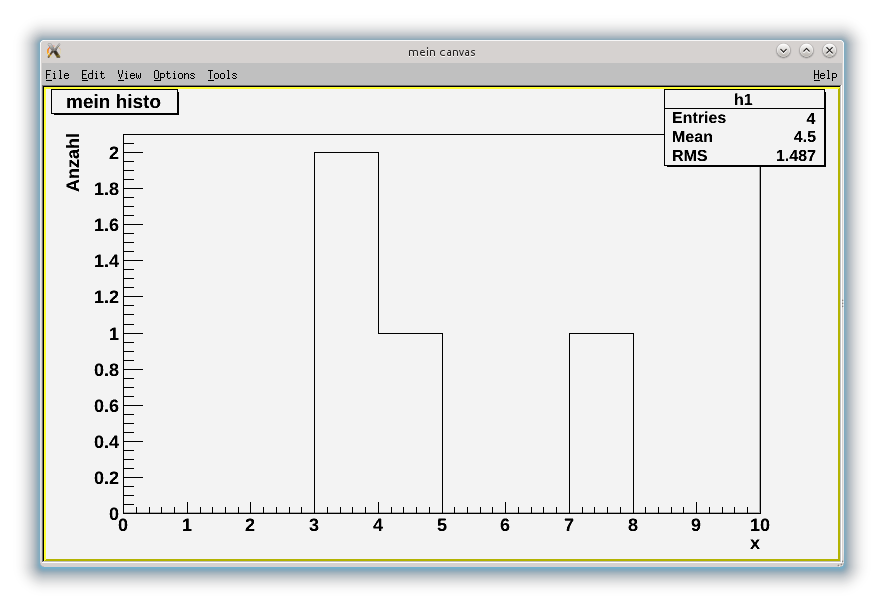
\includegraphics[width=10cm]{Uebung_10/default.png}
\caption{Standardplot}
\end{center}
\end{figure}



\begin{figure}[h]
\begin{center}
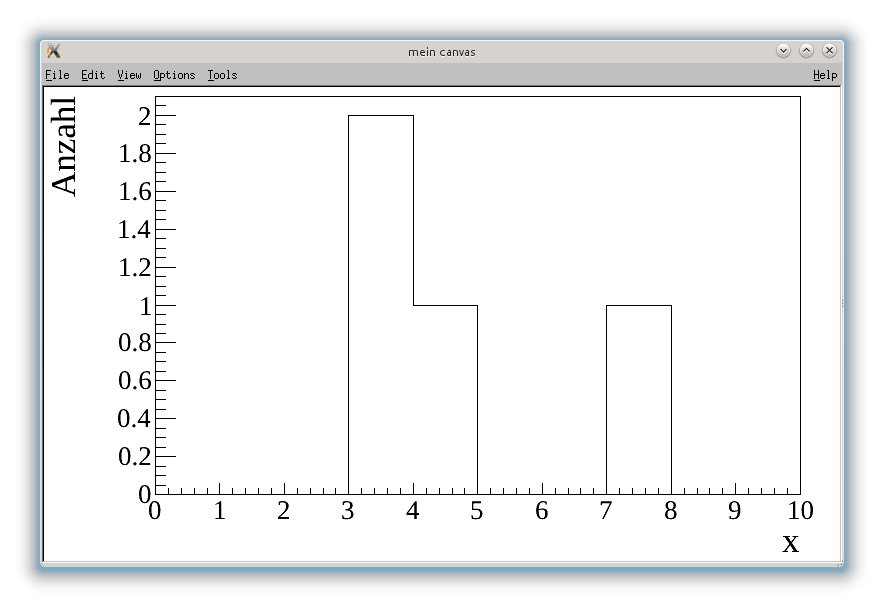
\includegraphics[width=10cm]{Uebung_10/babar.png}
\caption{BABAR Plot}
\end{center}
\end{figure}

Man kann mit \texttt{c1->SetLogx(1)} eine logarithmische Achse aktivieren und mit \texttt{c1->SetLogx(0)} wieder zurück zur linearen Achse wechseln.

\section{Berichtsaufgabe}

Man kann hier einfach den entsprechenden Konstruktor benutzen, da die Datei freundlichweise schon passend formatiert ist.

\code[c++]{Uebung_10/bericht.C}{Code fuer Plot}{code:root1}

ROOT gibt dann folgende Parameter für den Fit aus (Tablle \ref{table:fit}).

\begin{table}[h]
\begin{center}
\begin{tabular}{lcrcr}
Chi2 & = & $48.4851$ &  \\ 
NDf & = & $17$ &  \\ 
p0 & = & $-0.153455$ & $\pm$ & $0.0434887$ \\ 
p1 & = & $2.04459$ & $\pm$ & $0.00707916$ \\ 
\end{tabular} 
\caption{Parameter des Fits}
\label{table:fit}
\end{center}
\end{table}

ROOT zeichnet auch direkt die Linie ein. Man kann ihr Erscheinungsbild in der GUI dann auch noch verändern.


\begin{figure}[h]
\begin{center}
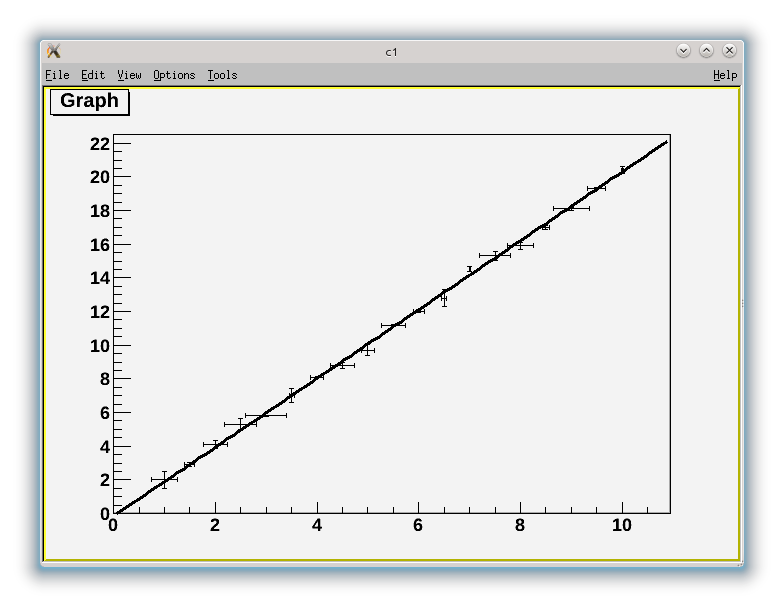
\includegraphics[width=10cm]{Uebung_10/fit.png}
\caption{Messwerte mit linearem Fit}
\end{center}
\end{figure}
